\documentclass[12pt]{article}


\usepackage{geometry}
 \geometry{
 a4paper,
 total={170mm,257mm},
 left=20mm,
 top=20mm,
 }


\usepackage{comment}
\usepackage{csquotes}

\usepackage{pgfplots}  
\usepgfplotslibrary{groupplots}
\usepackage{tikz}
\usetikzlibrary{decorations, arrows.meta, calligraphy}
\pgfplotsset{compat=newest}
\usepackage{amssymb}
\usepackage{bm}
\usepackage{MnSymbol}
\usepackage{siunitx}
\usepackage{xcolor}
\usepackage{lineno}

\usepackage{glossaries}
\newacronym{iga}{IGA}{iso-geometric analysis}


\DeclareMathOperator*{\argmin}{argmin}
\DeclareMathOperator{\Span}{span}


\definecolor{TUDa-0d}{cmyk/RGB/HTML}{0,0,0,.8/83,83,83/535353}
\definecolor{TUDa-0c}{cmyk/RGB/HTML}{0,0,0,.6/137,137,137/898989}
\definecolor{TUDa-0b}{cmyk/RGB/HTML}{0,0,0,.4/181,181,181/B5B5B5}
\definecolor{TUDa-0a}{cmyk/RGB/HTML}{0,0,0,.2/220,220,220/DCDCDC}
\definecolor{TUDa-10c}{cmyk/RGB/HTML}{.5,1,.3,0/149,17,105/951169}


\begin{document}
\title{Iso-Geometric Physics-Informed Neural Networks}
\maketitle
\section*{B-Splines and NURBs}
B-Splines or 'Basis-Splines' are a special type of spline which can be used for function approximation or as a basis functions in \gls{iga}.
A B-Spline of order $n$ is a piecewise polynomial of degree $n-1$ in a variable $x$.
To define the B-Spline knot vectors are necessary, which are simply given in the form
\begin{align}
\label{eq:knot_vector}
	\Xi = (\xi_0,\xi_1,...,\xi_N),
\end{align}
where $\xi_i\in\mathbb{R}$ and $\xi_i\leq\xi_j$ for $i\leq j$ i.e. the entries of the knot vectors are non-decreasing.
The first B-Spline is defined using \eqref{eq:knot_vector} as
\begin{align}
	B^{1}_i:=
	\begin{cases}
		1 \quad \text{for } \xi_i\leq x < \xi_{i+1} \\
		0 \quad \text{else}
	\end{cases}.
\end{align}
Higher-order B-Splines can be derived using the Cox-de-Boor recursion formula given as
\begin{align}
	B^{n+1}_i = \omega^k_i(x)B^k_i(x) + \left( 1- \omega^k_{i+1}(x) \right)B^k_{i+1}(x),
\end{align}
where
\begin{align}
	\omega^k_i(x):=
	\begin{cases}
		\frac{x-\xi_i}{\xi_{i+k}-\xi_i}\quad &\xi_{i+k}\neq \xi_i \\
		0 \quad &\text{else}
	\end{cases}.
\end{align}
To parametrize a curve with B-Splines, one has to define control points $\{\mathbf{c}_i\}_{i=1}^{N_c}\subset \mathbb{R}^2$ which warp the path of the curve.
The curve $C:\mathbb{R}\rightarrow \mathbb{R}^2$ is then given as an embedding
\begin{align}
\label{eq:curve}
	C(x) = \sum_{i=1}^{N_c}\mathbf{c}_i \,B_i^n(x).
\end{align} 
Similarly, parametrizations of surfaces can be constructed using tensor products of B-Spline curves.
In this case however, the B-Spline surface dependent on both spatial variables $x$ and $y$ and consequently $S:\mathbb{R}^2 \rightarrow \mathbb{R}^2$ with
\begin{align}
	S(x,y) = \sum_{j=1}^{N_c}\sum_{i=1}^{N_c}\mathbf{c}_{ij} \,B_i^n(x)B_j^n(y),
\end{align} 
where $\mathbf{c}_{ij}\in \mathbb{R}^2$ are points in a 2D control grid.
\subsection*{Differentiating B-Splines}
Here how to calculate the derivative and that derivatives of splines are again splines
\subsection*{Integrating over B-Splines}
To integrate over a B-Spline, one has to consider path integrals and transformation laws.
In the case we are considering a path integral along a B-Spline curve in $\mathbb{R}^2$, is given by
\begin{align}
\label{eq:bspline_path}
	I(f)=\int_{[0,1]} f\left( C(x)\right)\,\left|J_C\left(x\right)\right| \,\mathrm{d}x,
\end{align}
where $J_C$ is the jacobian of \eqref{eq:curve}.
The norm of the jacobian is given as 
\begin{align}
	\left|J_C(x) \right| = \sqrt{ \sum_{i=1}^{N_c} \left(\frac{\mathrm{d}B_i^n}{\mathrm{d}x}\left( x\right)\right)^2 \left(\mathbf{c}^2_{i,1} + \mathbf{c}^2_{i,2}\right)},
\end{align}
where $\mathbf{c}_{i} = (\mathbf{c}_{i,1}, \mathbf{c}_{i,2})$.
Generally, we evaluate \eqref{eq:bspline_path} using numerical quadrature.
An example of this would be Gauss-Legendre qaudrature, where we use quadrature points $X_q=\{x_1,...,x_{N_q}\}$ and weights $\Omega_q = \{\omega_1,...,\omega_{N_q}\}$ to approximate an integral via
\begin{align}
	I(f) = \int_{[-1,1]} f(x) \, \mathrm{d}x \approx \sum_{i=1}^{N_q} \omega_i \, f(x_i)
\end{align}
 For integrals over arbitrary domains $[a,b]$, one has to rescale the quadrature points and weights using the transformation
 \begin{align}
 	\overline{\omega}_i = \frac{b-a}{2} \omega_i\quad \text{and}\quad \overline{x}_i = \frac{b-a}{2}x_i + \frac{a+b}{2}.
 \end{align}
 As in the \gls{iga} framework, we typically parametrize the B-Splines over the unit cube and typically choose $a=0$ and $b=1$.
 Similarly, when integrating over a B-Spline surface, we evaluate
  \begin{align}
 	\int_{[0,1]^2} f\left(S(x,y)\right) \, \left|J_S(x,y) \right| \,\mathrm{d}x\mathrm{d}y \approx  \sum_{i=1}^{N_q} \sum_{j=1}^{N_q}  \omega_i \,\omega_j \, f\left(S(x_i,y_i) \right) \, \left|J_S(x_i,y_i) \right|,
 \end{align}
 where $\left|J_S(x_i,y_i) \right|$ denotes the jacobian determinant given by the formula
   \begin{align}
 	\left|J_S(x,y) \right| &= \left(\sum_{i=1}^{N_q}\sum_{j=1}^{N_q}\frac{\partial B^n_i}{\partial x}(x)B_i^n(y)\mathbf{c}_{i,1} \right) \left(\sum_{i=1}^{N_q}\sum_{j=1}^{N_q}B_i^n(x)\frac{\partial B^n_i}{\partial y}(y)\mathbf{c}_{i,2} \right) \\
 	&- \left(\sum_{i=1}^{N_q}\sum_{j=1}^{N_q}\frac{\partial B^n_i}{\partial x}(x) B_i^n(y)\mathbf{c}_{i,2} \right)\left(\sum_{i=1}^{N_q}\sum_{j=1}^{N_q} B_i^n(x)\frac{\partial B^n_i}{\partial y}(y)\mathbf{c}_{i,1} \right)
 \end{align}
 \newpage

\section*{Quadrupole Magnet}
\subsection*{Iron domain}

\begin{figure}
\centering
\begin{tikzpicture}
\node (cr) at (0,0){$\times$};

\coordinate (xmm) at (-3,-3);
\node[anchor = east] (xmm_l) at (-3.5,-3.5){$(-1,-1)$};

\coordinate (xpm) at ( 3,-3);
\node[anchor = west] (xpm_l) at (3.5,-3.5){$(1,-1)$};

\coordinate (xpp) at ( 3, 3);
\node[anchor = west] (xpm_l) at (3.5,3.5){$(1,1)$};

\coordinate (xmp) at (-3,3);
\node[anchor = east] (xpm_l) at (-3.5,3.5){$(-1,1)$};

\draw[purple, very thick] (xmm)--(xpm);
\draw[yellow, very thick] (xpm)--(xpp);
\node[anchor=north] (iron_iron) at ( 0, -3.25) {\textcolor{purple}{Iron - Iron 2 (14)}};

\draw[blue, very thick] (xpp)--(xmp);
\node[anchor=south] (pole_tip) at ( 0, 3.25){\textcolor{blue}{Iron - Air (12)}};
\node[anchor=south, rotate = -90] (32) at ( 3.25, 0){\textcolor{yellow}{Copper - Iron (31)}};
\node[anchor=south, rotate = 90] (dirichlet) at ( -3.25, 0){Dirichlet boundary};

\draw[very thick] (xmp)--(xmm);
\end{tikzpicture}
\end{figure}

\begin{itemize}
	\item \textcolor{blue}{Blue} Interface: Iron - Air, Label 12: $(y=1)$ $N(-1,1)$ is at the Dirichlet boundary condition. $N(1,1)$ is at the intersection of the domains $1,3,4$.
	\item \textcolor{purple}{Purple} Interface: Iron - Iron 2, Label 14: $(y=1)$ $N(1,-1)$ is at the intersection of the domains $1,2,3$. $N(-1,-1)$ is at the Dirichlet boundary 
     \item \textcolor{black}{Black} Dirichlet boundary condition at $N(-1,y)$
     \item \textcolor{yellow}{Yellow} Iron - Copper, Label 13: $(x=-1)$ $N(-1,y)$ is at the interface of iron yoke and the copper coil. $N(1,-1)$ is at the intersection of the domains $1,2,3$. $N(1,1)$ is at the intersection of the domains $1,3,4$.
\end{itemize}

\subsection*{Copper domain}

\begin{figure}
\centering
\begin{tikzpicture}
\node (cr) at (0,0){$\times$};

\coordinate (xmm) at (-3,-3);
\node[anchor = east] (xmm_l) at (-3.5,-3.5){$(-1,-1)$};

\coordinate (xpm) at ( 3,-3);
\node[anchor = west] (xpm_l) at (3.5,-3.5){$(1,-1)$};

\coordinate (xpp) at ( 3, 3);
\node[anchor = west] (xpm_l) at (3.5,3.5){$(1,1)$};

\coordinate (xmp) at (-3,3);
\node[anchor = east] (xpm_l) at (-3.5,3.5){$(-1,1)$};

\draw[gray, very thick] (xmm)--(xpm);
\draw[yellow,very thick] (xpm)--(xpp);
\node[anchor=north] (iron_iron) at ( 0, -3.25) {\textcolor{gray}{Copper - Iron 2 (34)}};
\node[anchor=south, rotate = 90] (dirichlet) at ( -3.25, 0){\textcolor{green}{Neumann boundary}};
\node[anchor=south, rotate = -90] (32) at ( 3.25, 0){\textcolor{yellow}{Copper - Iron (31)}};

\draw[blue, very thick] (xpp)--(xmp);
\node[anchor=south] (pole_tip) at ( 0, 3.25){\textcolor{blue}{Copper - Air (32)}};

\draw[green, very thick] (xmp)--(xmm);
\end{tikzpicture}
\end{figure}

\begin{itemize}
	\item \textcolor{blue}{Blue} Interface: Iron - Air, Label 12: $(y=1)$ $N(-1,1)$ is at the Dirichlet boundary condition. $N(1,1)$ is at the intersection of the domains $1,3,4$.
	\item \textcolor{yellow}{Yellow} Interface: Copper - Iron, Label 41: $(x=1)$ $N(1,-1)$ is at the intersection of the domains $1,2,3$. $N(1,1)$ is at the intersection of the domains $1,3,4$
     \item \textcolor{green}{Green} Neumann boundary condition at $N(-1,y)$
     \item \textcolor{gray}{Gray}: Copper - Iron 2, Label 24: $(y=-1)$ $N(x,-1)$ is at the interface of copper coil and the lower right iron yoke. $N(1,-1)$ is at the intersection of the domains $1,3,4$. $N(1,1)$ is at the lower right Dirichlet boundary condition.
\end{itemize}
Ansatz function for domain solution: $v(x,y) = (1-x)(1-y)(y+1)$

Interface functions:
\begin{itemize}
	\item $f_{31}(y) = \frac{1}{2}(y+1)(1-y)(1+y)$ and $f_{13}(x) = \frac{1}{2}(y+1)(1-y)(1+y)$
    \item $f_{32}(y) = \frac{1}{2} (x+1) (1-x)$  and $f_{34}(y) = -\frac{1}{2}(1-x)(x-1)$
    \item $f_{34}(x,y) = (1+x)(1+y)$ and 
\end{itemize}

\subsection*{Air domain}
\begin{figure}
\centering
\begin{tikzpicture}
\node (cr) at (0,0){$\times$};

\coordinate (xmm) at (-3,-3);
\node[anchor = east] (xmm_l) at (-3.5,-3.5){$(-1,-1)$};

\coordinate (xpm) at ( 3,-3);
\node[anchor = west] (xpm_l) at (3.5,-3.5){$(1,-1)$};

\coordinate (xpp) at ( 3, 3);
\node[anchor = west] (xpm_l) at (3.5,3.5){$(1,1)$};

\coordinate (xmp) at (-3,3);
\node[anchor = east] (xpm_l) at (-3.5,3.5){$(-1,1)$};

\draw[green, very thick] (xmm)--(xpm);
\draw[blue, very thick] (xpm)--(xpp);
\node[anchor=south, rotate = -90] (pole_tip) at ( 3.25, 0){\textcolor{blue}{Air - Iron (12)}};
\node[anchor=north] (neumann) at ( 0, -3.25) {\textcolor{green}{Neumann boundary}};

\draw[yellow, very thick] (xpp)--(xmp);
\node[anchor=south, rotate = 0] (pole_tip) at ( 0, 3.25){\textcolor{yellow}{Air - Copper (23)}};


\draw[very thick] (xmp)--(xmm);
\node[anchor=south, rotate = 90] (dirichlet) at ( -3.25, 0){Dirichlet boundary};
\end{tikzpicture}
\end{figure}

\begin{itemize}
	\item \textcolor{yellow}{Yellow} Interface: Air - Copper, Label 23: $(y=1)$ $N(-1,1)$ is at the Dirichlet boundary condition. $N(1,1)$ is at the intersection of the domains $1,2,3$.
	\item \textcolor{green}{Green} Neumann boundary condition $(y=-1)$ $N(1,-1)$ is at the Air - iron interface. $N(-1,-1)$ is at the origin.
     \item \textcolor{black}{Black} Dirichlet boundary condition at $N(-1,y)$
     
     \item \textcolor{blue}{Blue} Air - Iron, Label 13: $(x=1)$ $N(1,y)$ is at the interface of iron yoke and the air coil. $N(1,-1)$ is at the interface between the Iron pole and the air domain. $N(1,1)$ is at the intersection of the domains $1,2,3$.
\end{itemize}

\subsection*{Iron 2 domain}
\begin{figure}
\centering
\begin{tikzpicture}
\node (cr) at (0,0){$\times$};

\coordinate (xmm) at (-3,-3);
\node[anchor = east] (xmm_l) at (-3.5,-3.5){$(-1,-1)$};

\coordinate (xpm) at ( 3,-3);
\node[anchor = west] (xpm_l) at (3.5,-3.5){$(1,-1)$};

\coordinate (xpp) at ( 3, 3);
\node[anchor = west] (xpm_l) at (3.5,3.5){$(1,1)$};

\coordinate (xmp) at (-3,3);
\node[anchor = east] (xpm_l) at (-3.5,3.5){$(-1,1)$};

\draw[green, very thick] (xmm)--(xpm);
\draw[gray, very thick] (xpm)--(xpp);
\node[anchor=south, rotate = -90] (pole_tip) at ( 3.25, 0){\textcolor{gray}{Iron 2 - Copper (43)}};
\node[anchor=north] (dirichlet) at ( 0, -3.5) {\textcolor{green}{Neumann boundary}};

\draw[purple, very thick] (xpp)--(xmp);
\node[anchor=south, rotate = 0] (pole_tip) at ( 0, 3.25){\textcolor{purple}{Iron 2 - Iron (41)}};


\draw[very thick] (xmp)--(xmm);
\node[anchor=south, rotate = 90] (dirichlet) at ( -3.25, 0){Dirichlet boundary};
\end{tikzpicture}
\end{figure}

\begin{itemize}
	\item \textcolor{yellow}{Yellow} Interface: Iron 2 - Copper, Label 43: $(x=1)$ $N(1,-1)$ is at the Dirichlet boundary condition. $N(1,1)$ is at the intersection of the domains $1,3,4$.
	\item \textcolor{green}{Green} Dirichlet boundary condition $(y=-1)$ $N(1,-1)$ is at the Air - iron interface. $N(-1,-1)$ is at the lower right corner.
     \item Black: Dirichlet boundary condition at $N(-1,y)$
     
     \item \textcolor{blue}{Blue} Air - Iron, Label 13: $(x=1)$ $N(1,y)$ is at the interface of iron yoke and the air coil. $N(1,-1)$ is at the interface between the Iron pole and the air domain. $N(1,1)$ is at the intersection of the domains $1,2,3$.
\end{itemize}
Ansatz function for domain solution: $v(x,y) = (x+1)(1-x)(1-y)$
\begin{comment}
\begin{itemize}
	\item $u_{-1,-1}$ has $N_{-1,-1}(x,y) = (x+1) $
	\item $u_{-1,1}$ has $N_{-1,1}(x,y) = (x+1)f_{41}(y)= \frac{1}{2} (x+1)(x+1)$
    \item $u_{1,1}$ has $N_{1,1}(x,y) = f_{41}(y)f_{43}(x) =  \frac{1}{4} (x+1)(y+1)$ 
    \item $u_{1,-1}$ has $N_{1,-1}(x,y) = f_{43}(x)$ 
\end{itemize}
\end{comment}
Interface functions:
\begin{itemize}
	\item $f_{41}(x) = \frac{1}{2} (x+1)(1-x)(1+x)$ and $f_{14}(x) = -\frac{1}{2} (x-1)(1-x)(1+x)$
    \item $f_{43}(y) = \frac{1}{2} (x+1) (1-y)$  and $f_{34}(y) = -\frac{1}{2}(1-x)(x-1)$
    \item $f_{134}(x,y) = (1+x)(1+y)$ and 
\end{itemize}

\section*{Better Quadrupole}
\begin{tabular}{c|c}
		\hline \hline \\[-1.25ex]
		Pole Tip (\# 1) & Iron Yoke(\# 2) \\
		\hline
		
		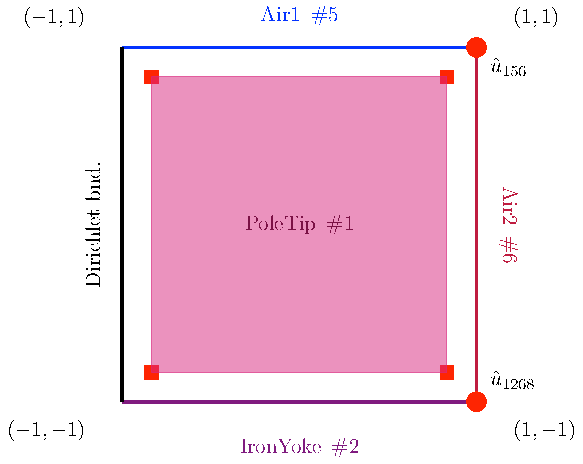
\includegraphics[width=0.5 \linewidth]{./standalones/PoleTip.pdf}
		&		 
		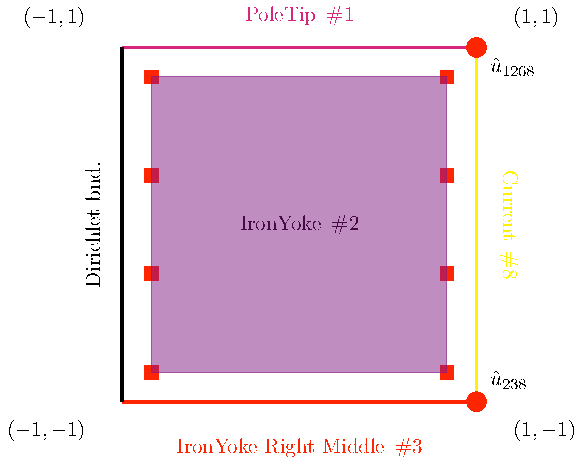
\includegraphics[width=0.5 \linewidth]{./standalones/IronYoke.pdf}
		\\
		\hline \\[-0.75ex]
		$B_{i,2}(x)$ with $\Xi = \left[-1,1\right]$ 
		& 
		$B_{i,2}(x)$ with $\Xi = \left[-1,1\right]$
		\\ [0.75ex]
		$B_{i,1}(y)$ with $\Xi = \left[-1,1\right]$ 
		& 
		$B_{i,1}(y)$ with $\Xi = \left[-1,-\frac{1}{3}, \frac{1}{3}, 1\right]$
		\\ [0.75ex]
		$v(x,y)=(x+1)(1-x)(y+1)(1-y)$ 
		&
		$v(x,y)=(x+1)(1-x)(y+1)(1-y)$
		\\ [0.75ex]
		\hline
		\\
		$f_{12}(x)=(x+1)(1-x) \, \cdot \, - \frac{1}{2}(y-1) \, u^{\tiny NN}_{12}(x)$
		&
		$f_{21}(x)= (x+1)(1-x) \, \cdot \,  \frac{1}{2}(y+1) \, u^{\tiny NN}_{12}(x)$
		\\ [0.75ex]
		$f_{15}(x)=(x+1)(1-x) \, \cdot \, \frac{1}{2}(y+1) \, u^{\tiny NN}_{15}(x)$
		&
		$f_{23}(x)=(x+1)(1-x)\, \cdot \,  -\frac{1}{2}(y-1) \, u^{\tiny NN}_{23}(x)$
		\\ [0.75ex]
		$f_{16}(x)=(y+1)(1-y)  \quad \cdot \quad \frac{1}{2}(x+1) \, u^{\tiny NN}_{16}(y)$ 
		&
		$f_{28}(x)=  (y+1)(1-y)  \, \cdot \, \left(\frac{1}{2}(x+1) \, u^{\tiny NN}_{28}(y)+ ...\right)$
		\\
		\hline
		\\ 
		$f_{156}(x,y)=\hat{u}_{156}\,((x+1)(y+1))^2$ 
		&
		$f_{1268}(x,y)=\hat{u}_{1268}\,((x+1)(y+1))^2$
		\\
		$f_{1268}(x,y)=\hat{u}_{1268}\,((x+1)(1-y))^2$ 
		&
		$f_{238}(x,y)=\hat{u}_{238}\,((x+1)(1-y))^2$
		\\
		\hline
		\hline
\end{tabular}
%
\begin{tabular}{c|c}
		\hline \hline \\[-1.25ex]
		Iron Yoke Right Middle (\# 3) & Iron Yoke Right Lower (\# 4) \\
		\hline
		\hline
		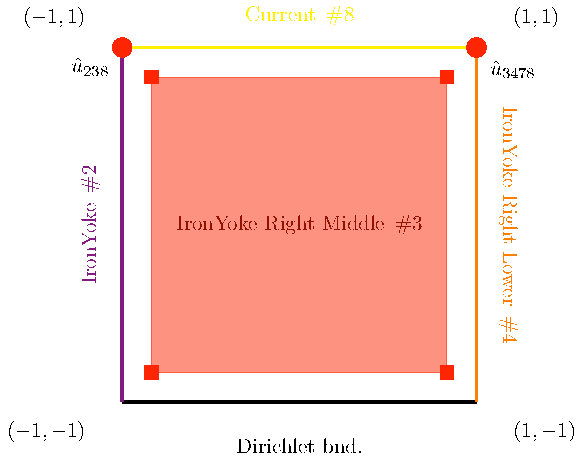
\includegraphics[width=0.5 \linewidth]{./standalones/IronYoke_Right_Middle.pdf} 
		&
		\includegraphics[width=0.5 \linewidth]{./standalones/IronYoke_Right_lower.pdf}		 
		\\
		\hline \\[-0.75ex]
		$B_{i,1}(x)$ with $\Xi = \left[-1,1\right]$ 
		& 
		$B_{i,1}(x)$ with $\Xi = \left[-1,1\right]$
		\\ [0.75ex]
		$B_{i,2}(y)$ with $\Xi = \left[-1,1\right]$
		& 
		$B_{i,2}(y)$ with $\Xi = \left[-1,1\right]$
		\\ [0.75ex]
		$v(x,y)=(x+1)(1-x)(y+1)(1-y)$ 
		&
		$v(x,y)=(x+1)(y+1)(1-y)$
		\\ [0.75ex]
		\hline
		\\ [-0.75ex]
		$f_{34}(x,y)= (y+1)(1-y) \, \cdot \, \frac{1}{2}(x+1) \,u^{\tiny NN}_{34}(y)$ 
		&
		$-$ 
		\\
		$f_{38}(x,y)= (x+1)(1-x) \, \cdot \, \frac{1}{2}(y+1) \,u^{\tiny NN}_{38}(x)$ 
		&
		$f_{47}(x,y)= (x+1) \, \cdot \, \frac{1}{2}(y+1) \,u^{\tiny NN}_{47}(x)$ 
		\\
		$f_{32}(x,y)= (y+1)(1-y) \, \cdot \, -\frac{1}{2}(x-1) \,u^{\tiny NN}_{23}(y)$ 
		&
		$f_{43}(x,y)= (y+1)(1-y) \, \cdot \, -\frac{1}{2}(x-1)\,u^{\tiny NN}_{34}(y)$ 
		\\ [0.75ex]
		\hline 
		\\ [-0.75ex]
		$f_{238}(x,y)=\hat{u}_{238}\,((1-x)(y+1))^2$ 
		&
		$-$
		\\
		$f_{3478}(x,y)=\hat{u}_{3478}\,((x+1)(y+1))^2$ 
		&
		$f_{3478}(x,y)=\hat{u}_{3478}\,((1-x)(y+1))^2$
		\\
		\hline
		\hline

\end{tabular}
	\newpage
\begin{tabular}{c|c}
		\hline \hline \\[-1.25ex]
		Air1 (\# 5) & Air2 (\# 6) \\
		\hline
		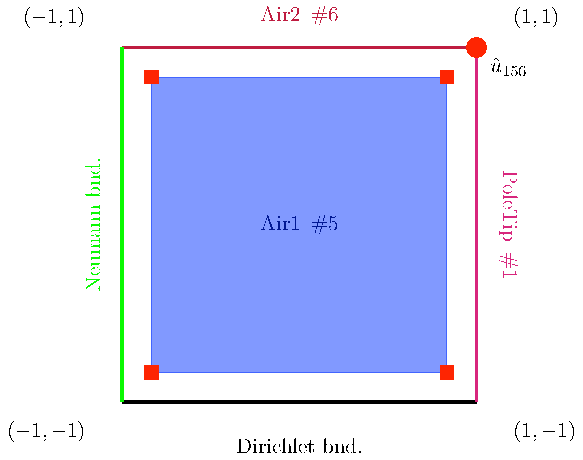
\includegraphics[width=0.5 \linewidth]{./standalones/Air1.pdf} &		 
		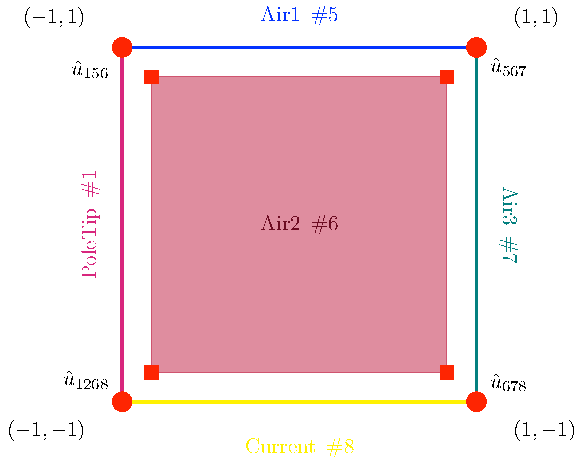
\includegraphics[width=0.5 \linewidth]{./standalones/Air2.pdf}
		\\
		\hline \\[-0.75ex]
		$B_{i,1}(x)$ with $\Xi = \left[-1,1\right]$ 
		& 
		$B_{i,1}(x)$ with $\Xi = \left[-1,1\right]$
		\\ [0.75ex]
		$B_{i,2}(y)$ with $\Xi = \left[-1,1\right]$
		& 
		$B_{i,1}(y)$ with $\Xi = \left[-1,1\right]$
		\\ [0.75ex]
		$v(x,y)=(1-x)(y+1)(1-y)$ 
		&
		$v(x,y)=(x+1)(1-x)(y+1)(1-y)$
		\\ [0.75ex]
		\hline
		\\ [-0.75ex]
		$f_{56}(x,y)= (1-x) \, \cdot \, \frac{1}{2}(y+1) \,u^{\tiny NN}_{56}(x)$ 
		&
		$f_{65}(x,y)= (x+1)(1-x) \, \cdot \, \frac{1}{2}(y+1) \,u^{\tiny NN}_{56}(x)$ 
		\\
		$f_{51}(x,y)= (y+1)(1-y) \, \cdot \, \frac{1}{2}(x+1) \,u^{\tiny NN}_{15}(y)$ 
		&
		$f_{67}(x,y)= (y+1)(1-y) \, \cdot \, \frac{1}{2}(x+1) \,u^{\tiny NN}_{67}(y)$ 
		\\
		$-$ 
		&
		$f_{68}(x,y)= (x+1)(1-x) \, \cdot \, -\frac{1}{2}(y-1)\,u^{\tiny NN}_{68}(x)$ 
		\\
		$-$ 
		&
		$f_{61}(x,y)= (y+1)(1-y) \, \cdot \, -\frac{1}{2}(x-1)\,u^{\tiny NN}_{16}(y)$ 
		\\ [0.75ex]
		\hline 
		\\ [-0.75ex]
		
		$f_{156}(x,y)=\hat{u}_{156}\,((x+1)(y+1))^2$ 
		&
		$f_{567}(x,y)=\hat{u}_{567}\,((x+1)(y+1))^2$
		\\
		$f_{567}(x,y) = \hat{u}_{567}\,((1-x)(y+1))^2$ 
		&
		$f_{678} = \hat{u}_{678}\,((x+1)(1-y))^2$
		\\
		$-$ 
		&
		$f_{1268} = \hat{u}_{1268}\,((1-x)(1-y))^2$
		\\
		$-$ 
		&
		$f_{156} = \hat{u}_{156}\,((1-x)(y+1))^2$
		\\
		\hline
		\hline
\end{tabular}


\begin{tabular}{c|c}
\hline \hline \\[-1.25ex]
		Air3 (\# 7) & Current (\# 8) \\
		\hline
		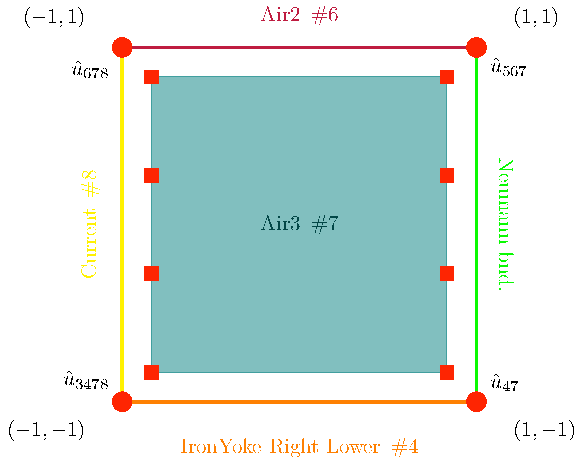
\includegraphics[width=0.5 \linewidth]{./standalones/Air3.pdf} &
		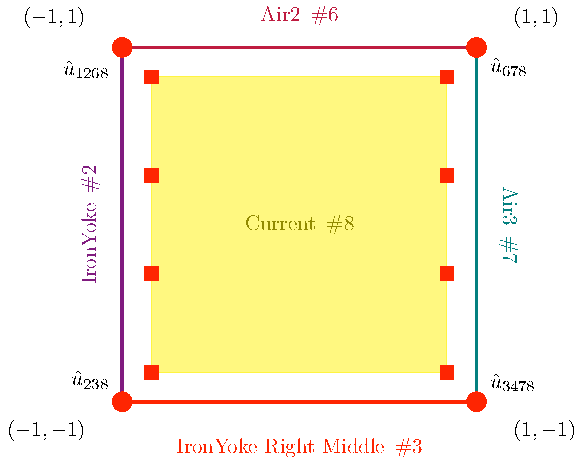
\includegraphics[width=0.5 \linewidth]{./standalones/Current.pdf}		 
		\\
		\hline \\[-0.75ex]
		$B_{i,1}(x)$ with $\Xi = \left[-1,1\right]$ 
		& 
		$B_{i,1}(x)$ with $\Xi = \left[-1,1\right]$
		\\ [0.75ex]
		$B_{i,1}(y)$ with $\Xi = \left[-1,-\frac{1}{3}, \frac{1}{3}, 1\right]$
		& 
		$B_{i,1}(y)$ with $\Xi = \left[-1,-\frac{1}{3}, \frac{1}{3}, 1\right]$
		\\ [0.75ex]
		$v(x,y)=(x+1)(y+1)(1-y)$ 
		&
		$v(x,y)=(x+1)(1-x)(y+1)(1-y)$
		\\ [0.75ex]
		\hline
		\\ [-0.75ex]
		$f_{76}(x,y)= (x+1) \, \cdot \, \frac{1}{2}(y+1) \,u^{\tiny NN}_{67}(x)$ 
		&
		$f_{86}(x,y)= (x+1)(1-x) \, \cdot \, \frac{1}{2}(y+1) \,u^{\tiny NN}_{68}(x)$ 
		\\
		
		$-$ 
		&
		$f_{87}(x,y)= (y+1)(1-y) \, \cdot \, \left(\frac{1}{2}(x+1) \,u^{\tiny NN}_{78}(y)+...\right)$ 
		\\
		$f_{74}(x,y)= (x+1) \, \cdot \, -\frac{1}{2}(y-1)\,u^{\tiny NN}_{47}(x)$ 
		&
		$f_{83}(x,y)= (x+1)(1-x) \, \cdot \, -\frac{1}{2}(y-1)\,u^{\tiny NN}_{38}(x)$ 
		\\
		$f_{78}= (y+1)(1-y) \, \cdot \, \left(-\frac{1}{2}(x-1)\,u^{\tiny NN}_{78}(y) + ...\right)$ 
		&
		$f_{82}= (y+1)(1-y) \, \cdot \, \left(-\frac{1}{2}(x-1)\,u^{\tiny NN}_{28}(y)+...\right)$ 
		\\ [0.75ex]
		\hline 
		\\ [-0.75ex]
		$f_{567}(x,y)=\hat{u}_{567}\,((x+1)(y+1))^2$ 
		&
		$f_{678}(x,y)=\hat{u}_{678}\,((x+1)(y+1))^2$
		\\
		$-$ 
		&
		$f_{3478} = \hat{u}_{3478}\,((x+1)(1-y))^2$
		\\
		$f_{3478} = \hat{u}_{3478}\,((1-x)(1-y))^2$ 
		&
		$f_{238} = \hat{u}_{238}\,((1-x)(1-y))^2$
		\\
		$f_{678} = \hat{u}_{678}\,((1-x)(y+1))^2$ 
		&
		$f_{1268} = \hat{u}_{1268}\,((1-x)(y+1))^2$
		\\
		\hline
		\hline
	\end{tabular}

\end{document}

